%!TEX program = xelatex
\documentclass[cn,normal,black,11pt]{elegantnote}
\usepackage{wasysym}
\usepackage{multirow}
% \title{ElegantNote:一个优美的 \LaTeX{} 笔记模板}

% \author{\href{https://ddswhu.me/}{邓东升}}
% \institute{\href{https://elegantlatex.org/}{Elegant\LaTeX{} Program}}
% \version{2.20}
% \date{\today}


\begin{document}
% \newcommand{\stuname}{吕昱峰}
% \newcommand{\stuclass}{2017级计算机科学与技术(卓越)01班}
% \newcommand{\expname}{实验四 简单五级流水线CPU}
% \newcommand{\expdate}{2019 年 11 月 8 日}
% \newcommand{\reportdate}{\number\year 年 \number\month 月 \number\day 日}
% \newcommand{\exproom}{A主404}
% \newcommand{\stugrade}{优秀/良好/中等}
% \newcommand{\teacher}{钟将}
% \newcommand{}{}

\newcommand{\stunameone}{曹仕20221444}
\newcommand{\stunametwo}{胡俊伦20221555}
\newcommand{\stuclass}{2022级计算机科学与技术(卓越)01班}
\newcommand{\expname}{实验四 简单五级流水线CPU}
\newcommand{\expdate}{2024 年 4 月 19 日}
\newcommand{\reportdate}{\number\year 年 \number\month 月 \number\day 日}
\newcommand{\exproom}{DS1410}
\newcommand{\stugrade}{优秀/良好/中等}
\newcommand{\teacher}{钟将}

% \maketitle
% logo
% \centerline{
\includegraphics[width=0.25\textwidth]{logo.pdf}}

\setlist[itemize]{label=$\circ$}

\centerline{\textbf{\huge{《计算机组成原理》实验报告}}}


\begin{table}[htbp]
    \centering
    \begin{tabular}{|c|c|c|c|}
        \hline
        \multirow{2}{*}{\textbf{年级、专业、班级}} & \multirow{2}{*}{\stuclass} & \multirow{2}{*}{\textbf{姓名}} & \stunameone  \\ 
        &  &  &  \stunametwo \\ \hline
         \textbf{实验题目} & \multicolumn{3}{c|}{\expname} \\ 
         \hline
         \textbf{实验时间} & \expdate & \textbf{实验地点} & \exproom \\ \hline
\multirow{3}{*}{\textbf{实验成绩}} & \multirow{3}{*}{\stugrade} & \multirow{3}{*}{\textbf{实验性质}} & \Square{验证性}  \\
         &  &  &  \CheckedBox{设计性}\\
         &  &  &  \Square{综合性} \\ \hline
         \multicolumn{4}{|l|}{\textbf{教师评价:}} \\
         \multicolumn{4}{|c|}{\Square{算法/实验过程正确;}\quad \Square{源程序/实验内容提交; }\quad \Square{程序结构/实验步骤合理; } }\\
         \multicolumn{4}{|c|}{\Square{实验结果正确;}\quad\quad\quad \Square{语法、语义正确;}\quad\quad \Square{报告规范;} }\\
         \multicolumn{4}{|l|}{其他:} \\
         \multicolumn{4}{|r|}{评价教师: \teacher} \\ \hline
         \multicolumn{4}{|l|}{\textbf{实验目的}} \\
         \multicolumn{4}{|l|}{(1)掌握流水线(Pipelined)处理器的思想。} \\
         \multicolumn{4}{|l|}{(2)掌握单周期处理中执行阶段的划分。} \\
         \multicolumn{4}{|l|}{(3)了解流水线处理器遇到的冒险。} \\
         \multicolumn{4}{|l|}{(4)掌握数据前推、流水线暂停等冒险解决方式。} \\ \hline
         
    \end{tabular}
    % \caption{Caption}
    \label{tab:my_label}
\end{table}

报告完成时间: \reportdate


\newpage

% \section{实验内容}
阅读实验原理实现以下模块:
\begin{enumerate}[(1)]
    \item Datapath,所有模块均可由实验三复用,需根据不同阶段,修改mux2为mux3(三选一选择器),以及带有enable(使能)、clear(清除流水线)等信号的触发器,
    \item Controller,其中main decoder与alu decoder可直接复用,另需增加触发器在不同阶段进行信号传递
    \item 指令存储器inst\_mem(Single Port Ram),数据存储器data\_mem(Single Port Ram);同实验三一致,无需改动,
    \item 参照实验原理,在单周期基础上加入每个阶段所需要的触发器,重新连接部分信号。实验给出top文件,需兼容top文件端口设定。
    \item 实验给出仿真程序,最终以仿真输出结果判断是否成功实现要求指令。
\end{enumerate}

% \section{实验设计}
% \textcolor{red}{这一节,主要描述各个模块的功能、接口、逻辑控制方法(状态机控制方法)等。(红字为内容说明,请删除)}
\subsection{单周期改流水线原理}
实验三已完成图中单周期的部分,可以看到,流水线处理器的主要改动,是在每个执行阶段
加入触发器,使得每个周期执行一个阶段,得到的结果送往下一个周期进行执行,同时下一条指
令执行一个阶段,这样能够使指令各阶段并行执行,提升效率。
\begin{figure}[H]
	\centering
	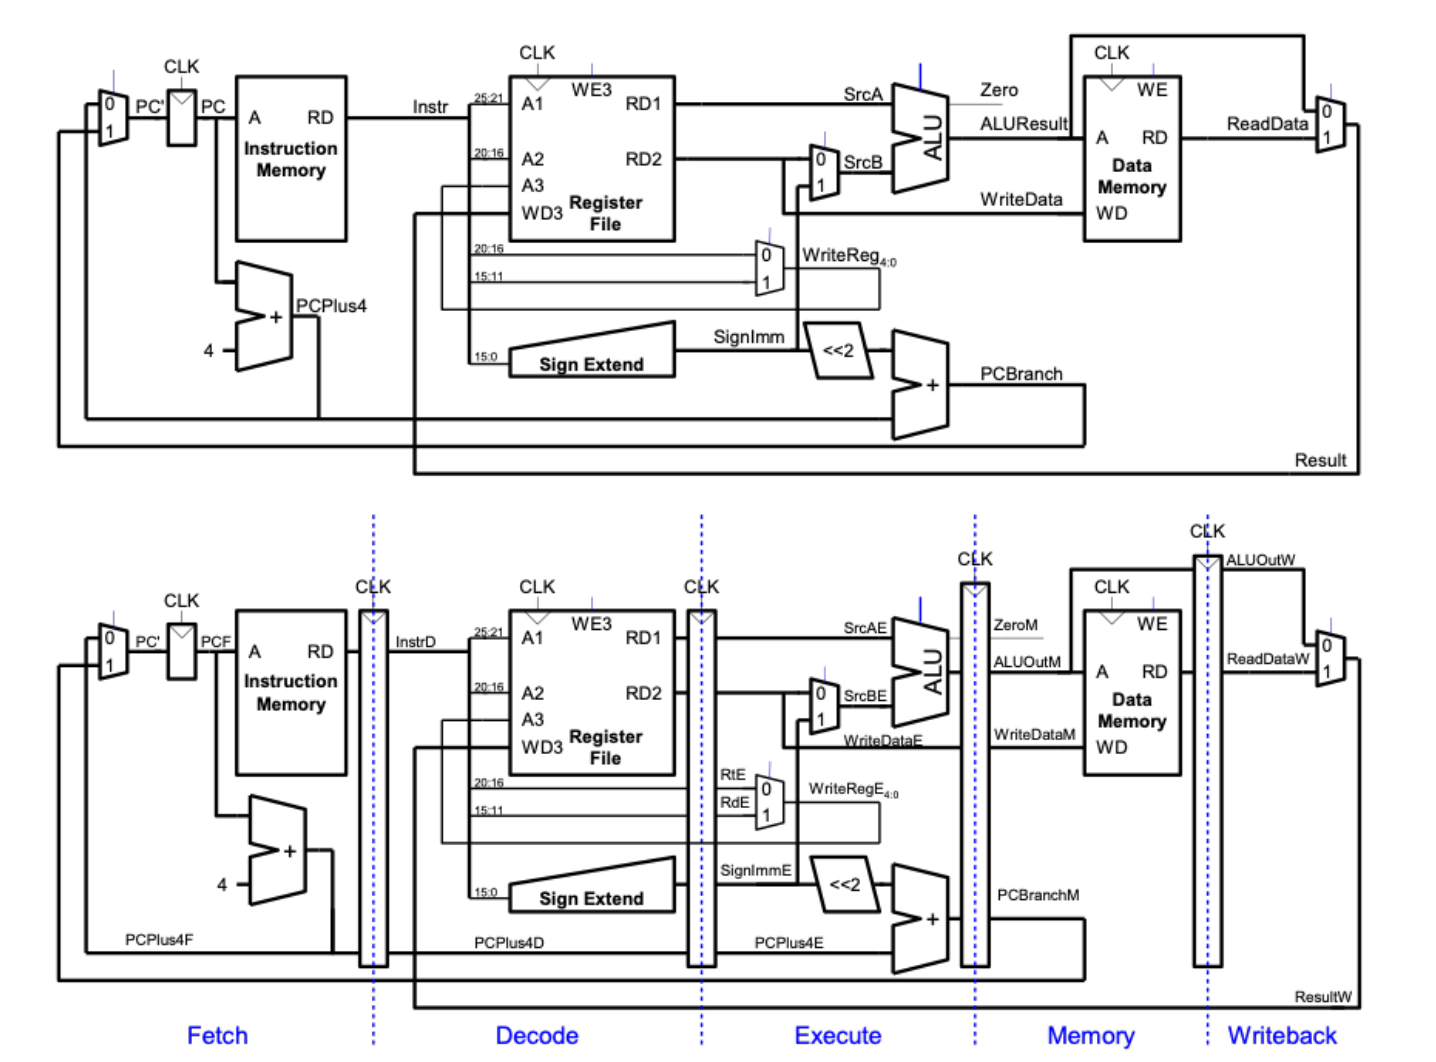
\includegraphics[width=0.75\textwidth]{figure/单周期和流水线比较.png}
	\caption{单周期和流水线比较}
	\label{fig:single_cycle_pipeline}
\end{figure}
可以看到,单周期中写寄存器堆的地址信号 writereg 需要延迟到 writeback 阶段与回写数据
result 一起写回寄存器堆:
\begin{figure}[H]
	\centering
	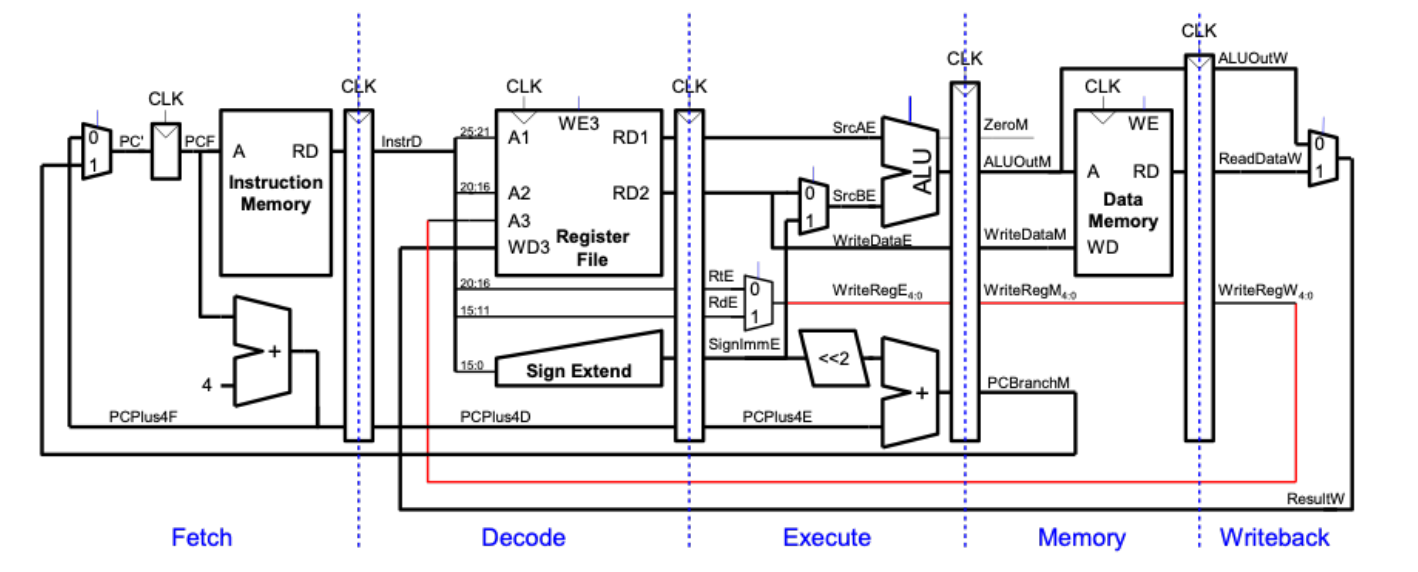
\includegraphics[width=0.75\textwidth]{figure/修改writereg信号.png}
	\caption{修改writereg信号}
	\label{fig:modify_writereg}
\end{figure}
在此基础上,datapath 的基本通路已经形成,下面加入控制器部分。控制器部分与单周期相
同,仍然由 main decoder 和 alu decoder 构成,但由于改为五级流水线后,每一个阶段所需要的控
制信号仅为一部分,控制器产生信号的阶段为译码阶段,产生控制信号后,依次通过触发器传到
下一阶段,若当前阶段需要的信号,则不需要继续传递到下一阶段:
\begin{figure}[H]
	\centering
	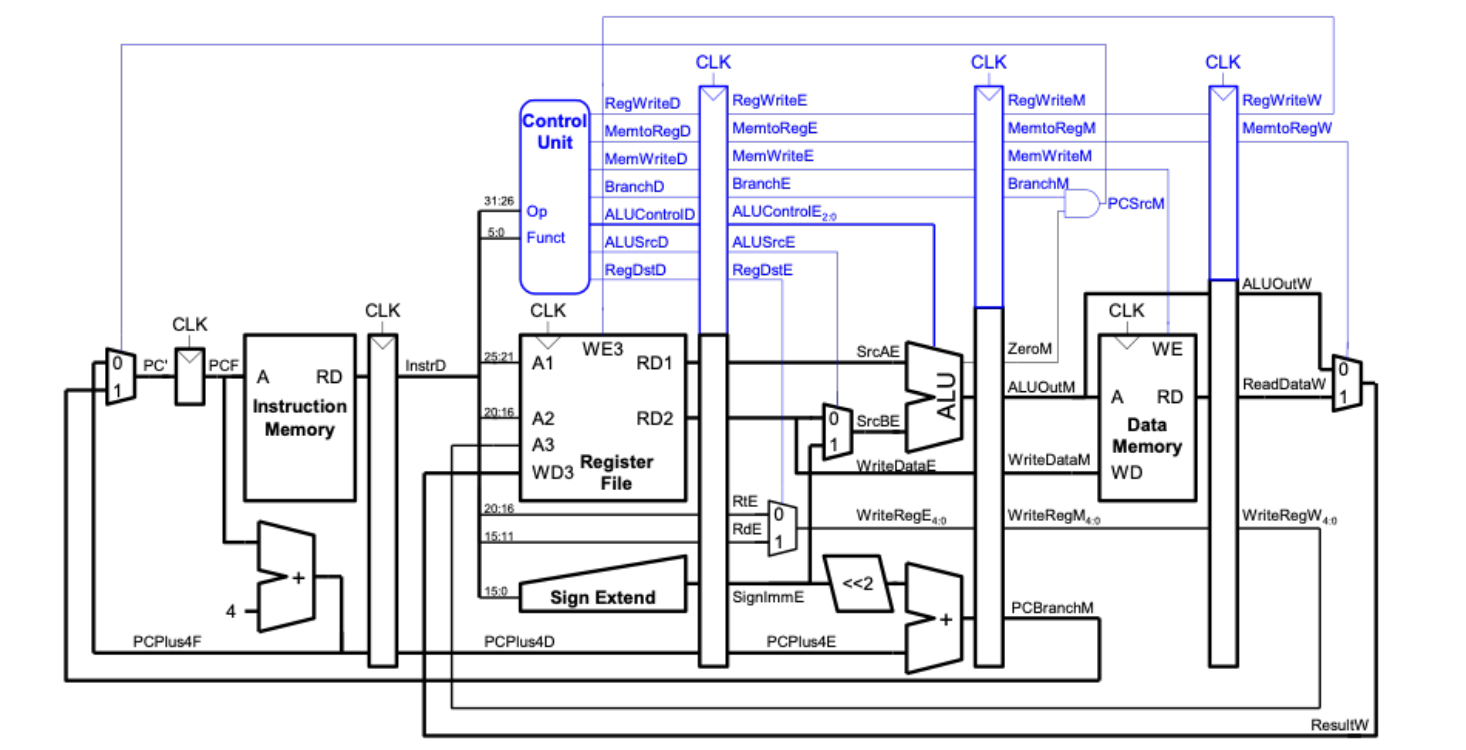
\includegraphics[width=0.75\textwidth]{figure/加入控制器的流水线示意图.png}
	\caption{加入控制器的流水线示意图}
	\label{fig:pipeline_with_controller}
\end{figure}
\subsection{各类型触发器的实现}
实验三中已给出触发器 flopr,作为 PC 使用,此外需要在其基础上实现下列触发器:

(1)flopr:带有 reset 的触发器

(2)floprc:带有 reset 与 clear 的触发器

(3)flopenrc:带有 enable、reset 与 clear 的触发器

flopr 的写法如下:
\begin{lstlisting}[language=Verilog,caption={flopr实现},label={lst:flopr}]

	module flopenr #(parameter WIDTH = 32)
					(input clk,
					 input rst,
					 input en,
					 input [WIDTH-1:0] d,
					 output reg [WIDTH-1:0] q);
		
	always @(posedge clk, posedge rst) begin
		if (rst) begin
			q <= 0;
		end else if (en) begin
			q <= d;
		end
	end
		
	endmodule
		
	
\end{lstlisting}

floprc 的写法如下:
\begin{lstlisting}[language=Verilog,caption={floprc实现},label={lst:floprc}]
module floprc #(parameter WIDTH = 8)
				(input wire clk, rst, clear,
				input wire [WIDTH -1:0] d,
				output reg [WIDTH -1:0] q);

	always @(posedge clk , posedge rst) begin
		if (rst) begin
			q <= 0;
		end else if (clear) begin
			q <= 0;
		end else begin
			q <= d ;
		end
	end

endmodule

\end{lstlisting}
flopenrc 的写法如下:

\begin{lstlisting}[language=Verilog,caption={flopenrc实现},label={lst:flopenrc}]
module flopenrc #(parameter WIDTH = 8)
                 (input wire clk,
                  rst,
                  en,
                  clear,
                  input wire [WIDTH -1:0] d,
                  output reg [WIDTH -1:0] q);
    
    always @(posedge clk) begin
        if (rst) begin
            q <= 0;
        end else if (clear) begin
            q <= 0;
        end else if (en) begin
            /* code */
            q <= d;
        end
    end

endmodule

\end{lstlisting}
\subsection{冒险处理模块}\label{sub:hazard}
在流水线 CPU 中,并不是能够完全实现并行执行,常见的冲突有竞争和冒险。竞争是门电路
两个输入信号同时向相反方向的逻辑电平跳变而导致的现象,本实验不作处理。而对于冒险,在
单周期中由于每条指令执行完毕才会执行下一条指令,并不会遇到冒险问题,而在流水线处理器
中,由于当前指令可能取决于前一条指令的结果,但此时前一条指令并未执行到产生结果的阶段,
这时候,就产生了冒险。本实验设计 hazard 模块处理冒险。

冒险分为:

1. 数据冒险:寄存器中的值还未写回到寄存器堆中,下一条指令已经需要从寄存器堆中读取
数据;

2. 控制冒险:下一条要执行的指令还未确定,就按照 PC 自增顺序执行了本不该执行的指令
(由分支指令引起)。
\subsubsection{功能描述}
1. 数据冒险:
如图 1 中指令,and、or、sub 指令均需要使用 \$s0 中的数据,然而 add 指令在回写阶段才能写
入寄存器堆,此时后续三条指令均已经过或正在执行译码阶段,得到的结果均为错误值。以上就
是数据冒险的特点,数据冒险有以下解决方式:

(1)在编译时插入空指令;

(2)在编译时对指令执行顺序进行重排;

(3)在执行时进行数据前推;

(4)在执行时,暂停处理器当前阶段的执行,等待结果。
\begin{figure}[H]
	\centering
	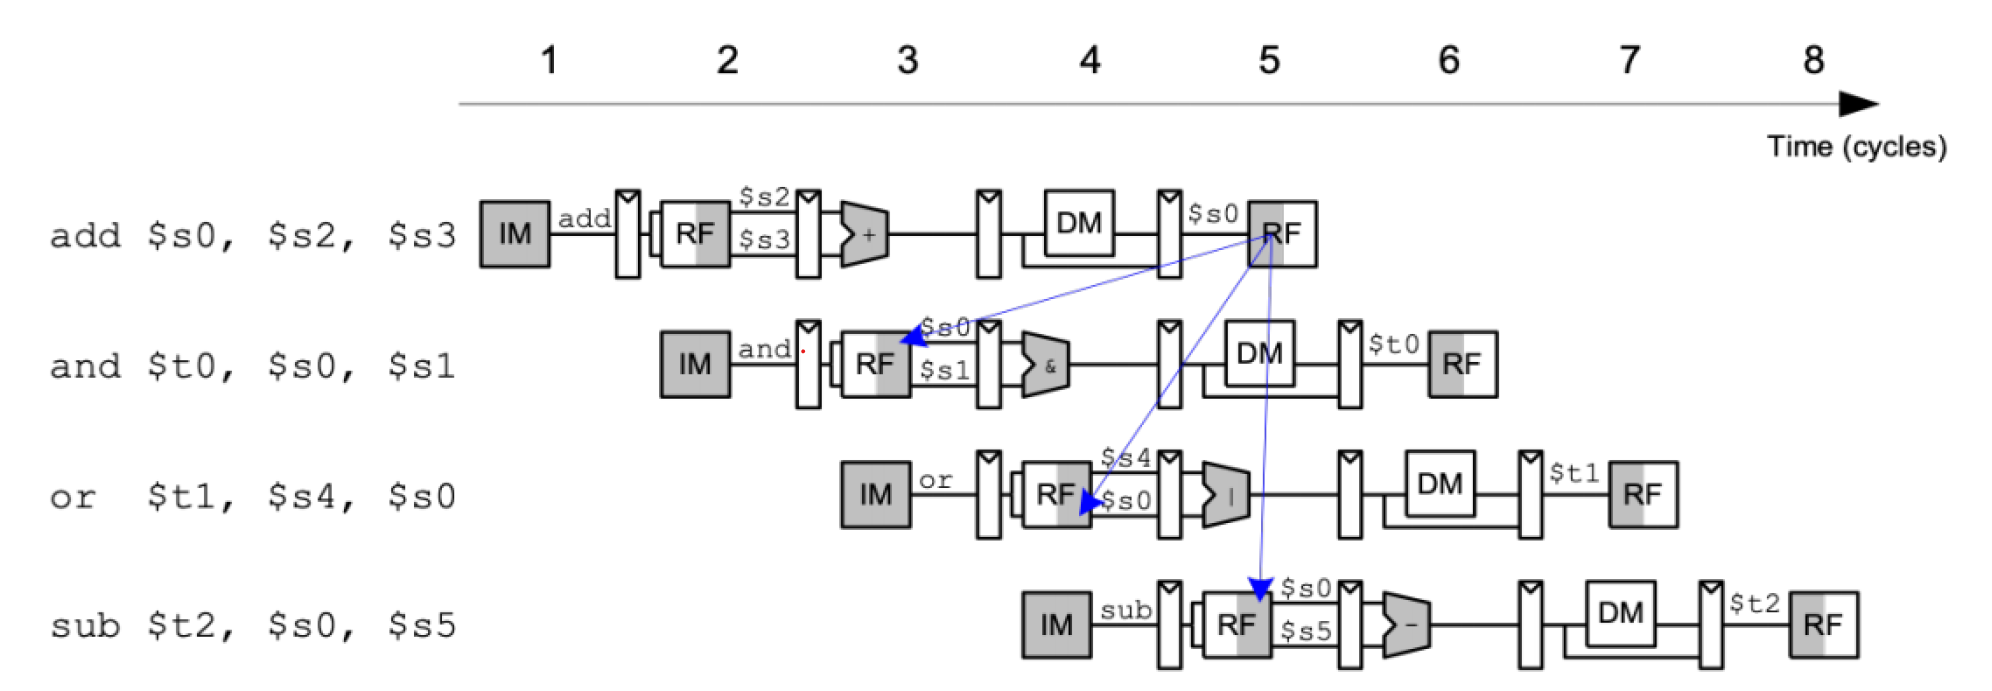
\includegraphics[width=0.75\linewidth]{figure/数据冒险示例.png}
	\caption{数据冒险示例}
	\label{fig:data_hazard}
	\end{figure}

但由于我们未进行指令编译层的处理,因此只需要在运行时 (run time) 进行解决,故采用数
据前推和暂停处理器两种解决方案。

1.1 数据前推

从图 5 所示,add 指令的结果在 execute 阶段已经由 ALU 计算得到,此时可以将 alu 得到的结
果直接推送到下一条指令的 execute 阶段,同理,后续所有的阶段均已有结果,可以向对应的阶段
推送,而不需要等到回写后再进行读取,达到数据前推的目的。
% \textcolor{red}{简单描述实现的功能即可,一句话亦可(红字为内容说明,请删除)}
\begin{figure}[ht]
	\centering
	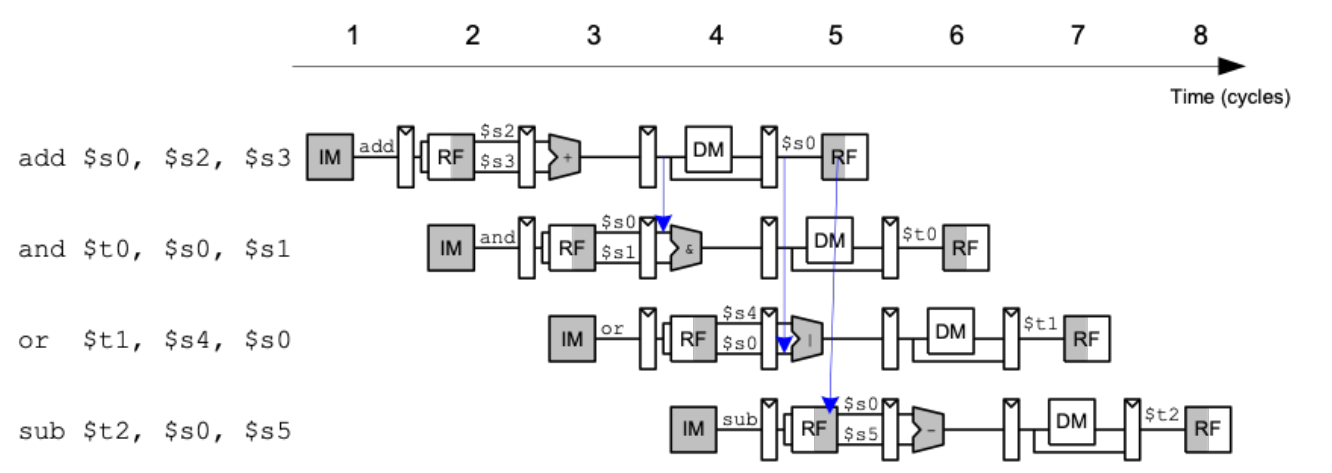
\includegraphics[width=0.75\linewidth]{figure/数据前推示例.png}
	\caption{数据前推示例}
	\label{fig:data_forward_example}
	\end{figure}

从图 5 中可以看到,add 指令的结果在 execute 阶段已经由 ALU 计算得到,此时可以将 alu 得
到的结果直接推送到下一条指令的 execute 阶段,同理,后续所有的阶段均已有结果,可以向对应
的阶段推送,而不需要等到回写后再进行读取,达到数据前推的目的。

数据前推的实现逻辑如下:	
\begin{lstlisting}[language=Verilog,caption={数据前推},label={lst:data_forward}]
	assign forwardAE = ((rsE != 0) && (rsE == writeregM) && regwriteM) ? 2'b10 :
                   ((rsE != 0) && (rsE == writeregW) && regwriteW) ? 2'b01 :
                   2'b00;
	assign forwardBE = ((rtE != 0) && (rtE == writeregM) && regwriteM) ? 2'b10 :
                   ((rtE != 0) && (rtE == writeregW) && regwriteW) ? 2'b01 :
                   2'b00;

\end{lstlisting}

在 execute 阶段需要判断当前输入 ALU 的地址是否与其他指令在此时
执行的阶段要写入寄存器堆的地址相同,如果相同,就需要将其他指令的结果直接通过多路选择
器输入到 ALU 中。

此处需要:

1. 增加 rs,rt 的地址传递到 execute 阶段,并与冒险模块连接;

2. Memory 阶段和 writeback 阶段要写入寄存堆的地址与冒险模块连接;

3. Memory 阶段和 writeback 阶段的寄存器堆写使能信号 regwrite 与冒险模块连接;

4. 根据实现逻辑,将生成的 forward 信号输出,控制 mux3 选择器。

数据通路结构如下:
\begin{figure}[H]
	\centering
	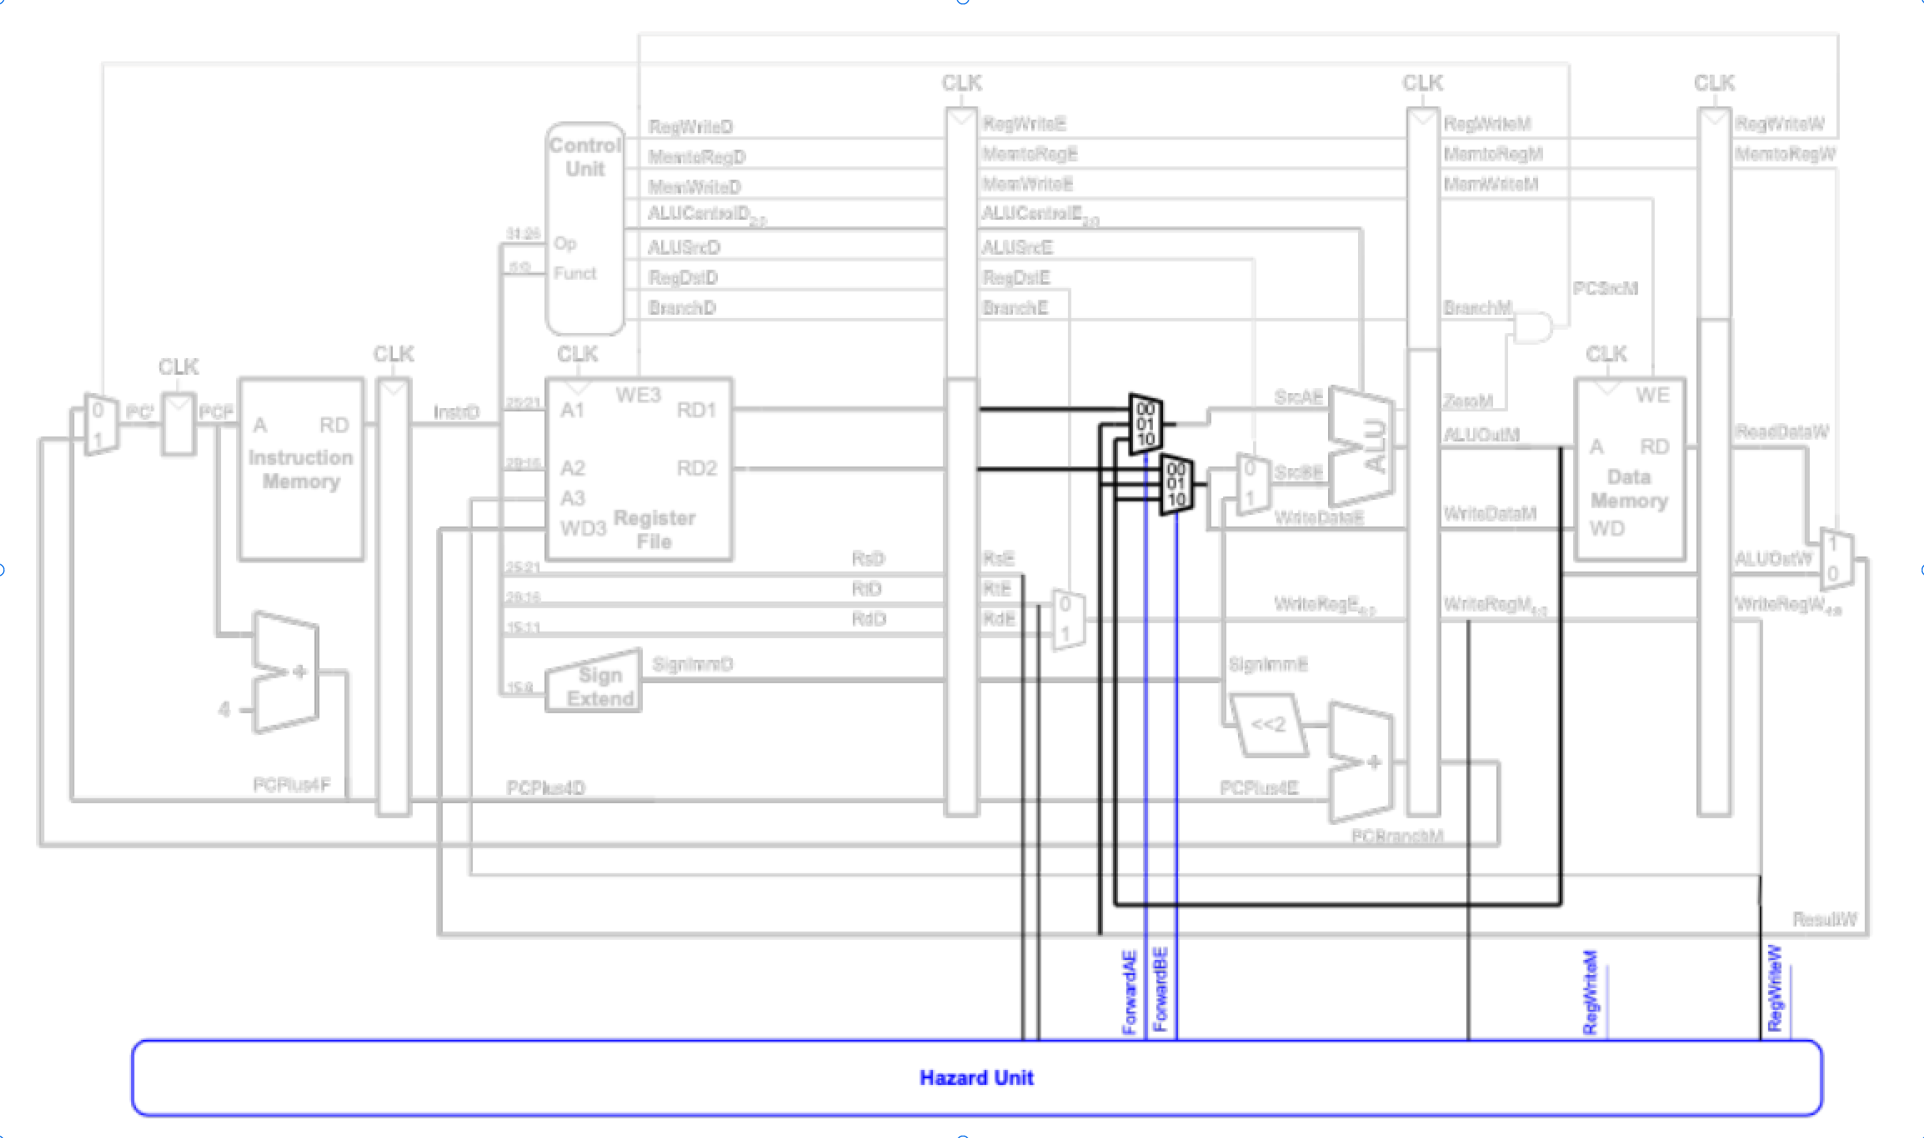
\includegraphics[width=0.75\textwidth]{figure/加入数据前推的数据通路结构.png}
	\caption{加入数据前推的数据通路结构}
	\label{fig:data_forward_data_path}
\end{figure}

1.2 流水线暂停
多数情况下,数据前推能解决很大一部分数据冒险的问题,然而在图中 7,lw 指令在 memory
阶段才能够从数据存储器读取数据,此时 and 指令已经完成 ALU 计算,无法进行数据前推。

如图 8在这种情况下,必须使流水线暂停,等待数据读取后,再前推到 execute 阶段。
\begin{figure}[H]
	\centering
	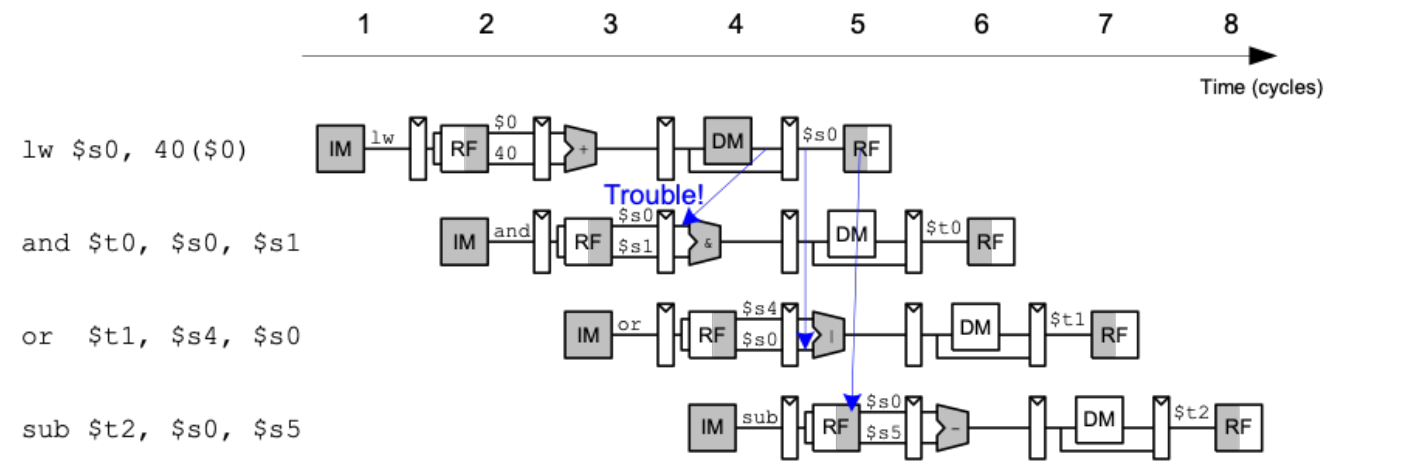
\includegraphics[width=0.75\textwidth]{figure/数据无法前推的情况.png}
	\caption{数据无法前推的情况}
	\label{fig:data_forward_stall}
\end{figure}

\begin{figure}[H]
	\centering
	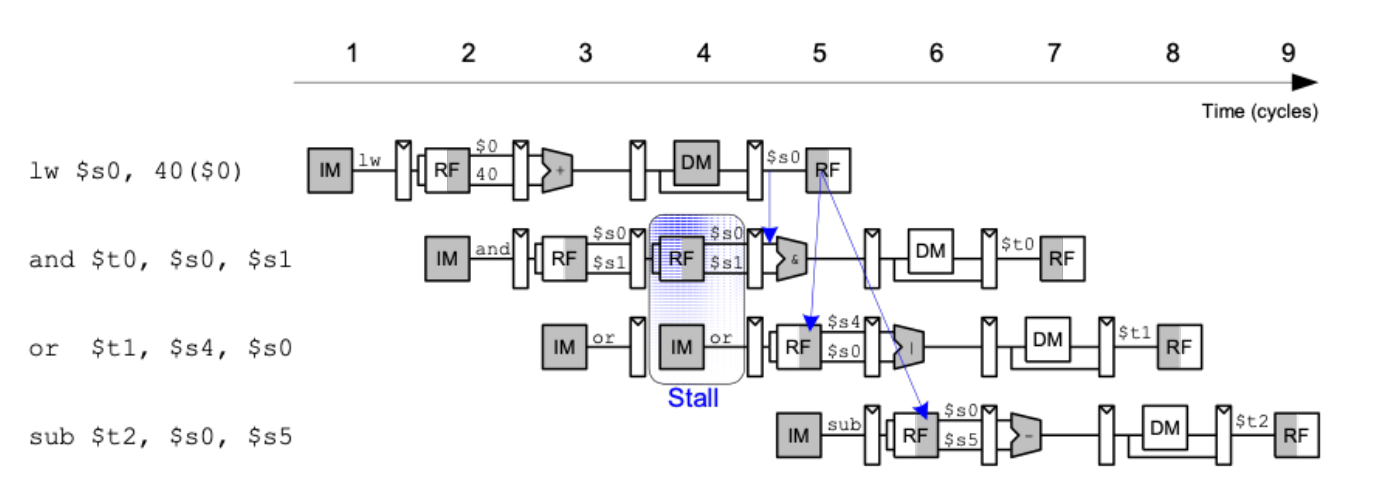
\includegraphics[width=0.75\textwidth]{figure/流水线暂停示例.png}
	\caption{流水线暂停示例}
	\label{fig:data_forward_stall_example}
\end{figure}
流水线暂停的条件是:前一条指令需要对寄存器堆写入 (memturegE=1) 并且写入地址 rtE 与
被当前指令用 (rsD==rtE 或 rtD==rtE)。并且该暂停信号会将后几级流水线全部暂停。注意,流水
线暂停 (decoder 级) 还需要一个附加操作,就是清空 excute 级的信号。因为 lw 下一条指令已经按
照预期接受了流水寄存器 DE 的输出并进行工作。到下面介绍的控制冒险也会用到流水线暂停,
因此将流水线暂停的数据通路和逻辑控制放在控制冒险后介绍。

2. 控制冒险:

控制冒险是分支指令引起的冒险。在五级流水线当中,分支指令在第 4 阶段才能够决定是否
跳转;而此时,前三个阶段已经导致三条指令进入流水线开始执行,这时需要将这三条指令产生
的影响全部清除。
\begin{figure}[H]
	\centering
	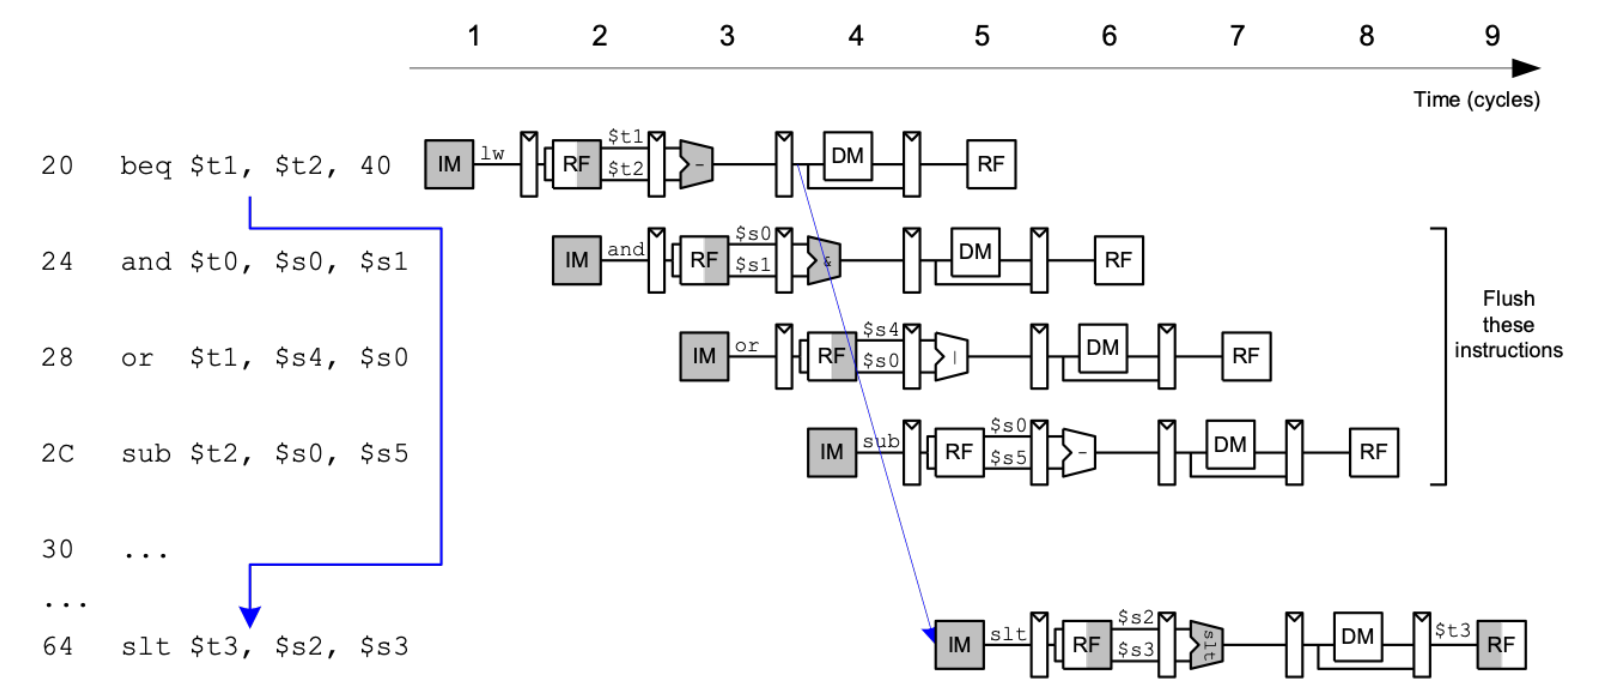
\includegraphics[width=0.75\textwidth]{figure/控制冒险示例.png}
	\caption{控制冒险示例}
	\label{fig:control_hazard}
\end{figure}
将分支指令的判断提前至 decode 阶段,此时能够减少两条指令的执行;
\begin{figure}[H]
	\centering
	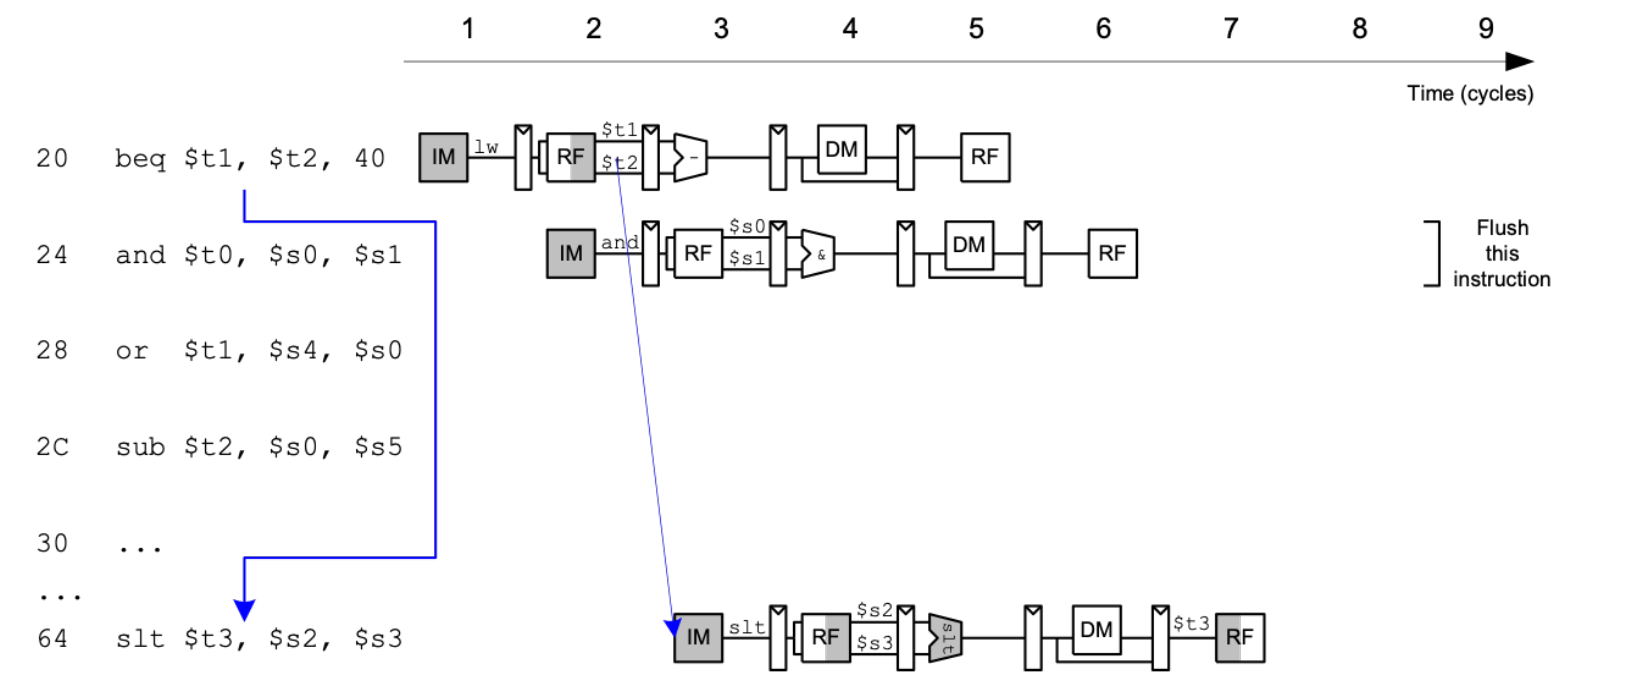
\includegraphics[width=0.75\textwidth]{figure/提前判断分支.png}
	\caption{提前判断分支}
	\label{fig:control_hazard_forward}
\end{figure}
在 regfile 输出后添加一个判断相等的模块,即可提前判断 beq:
\begin{figure}[H]
	\centering
	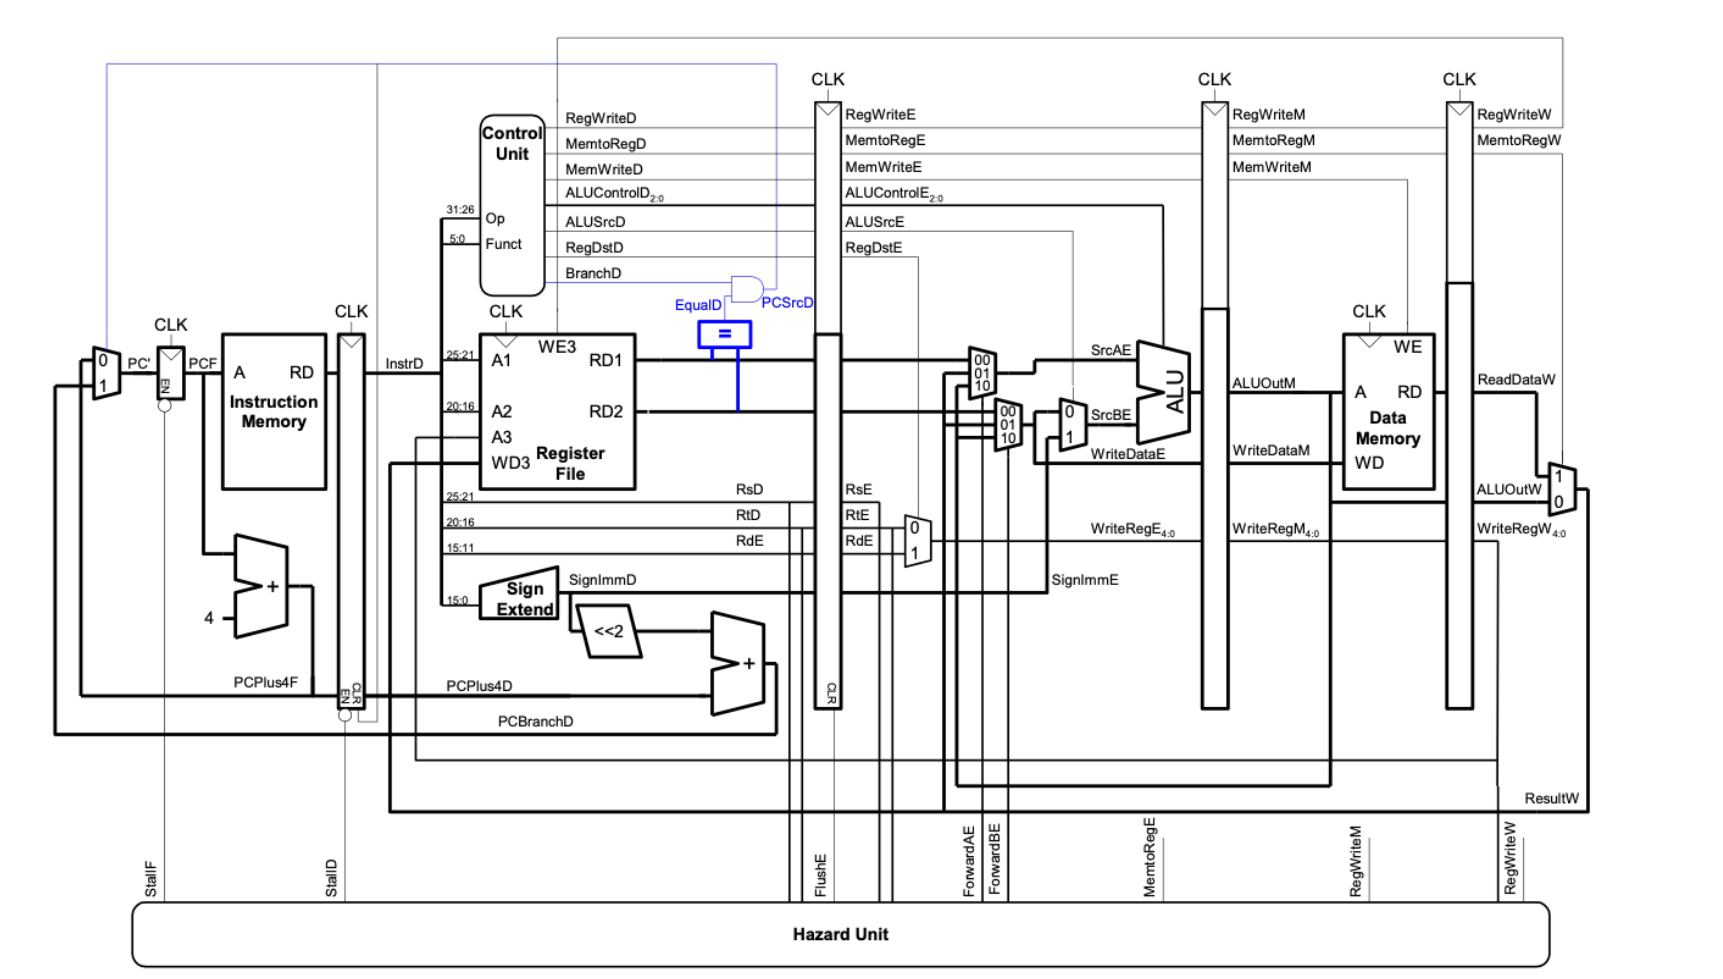
\includegraphics[width=0.75\textwidth]{figure/提前判断分支的实现.png}
	\caption{提前判断分支的实现}
	\label{fig:control_hazard_forward_implementation}
\end{figure}
此时又产生了数据冲突问题,需要增加数据前推和流水线暂停模块;
\begin{figure}[H]
	\centering
	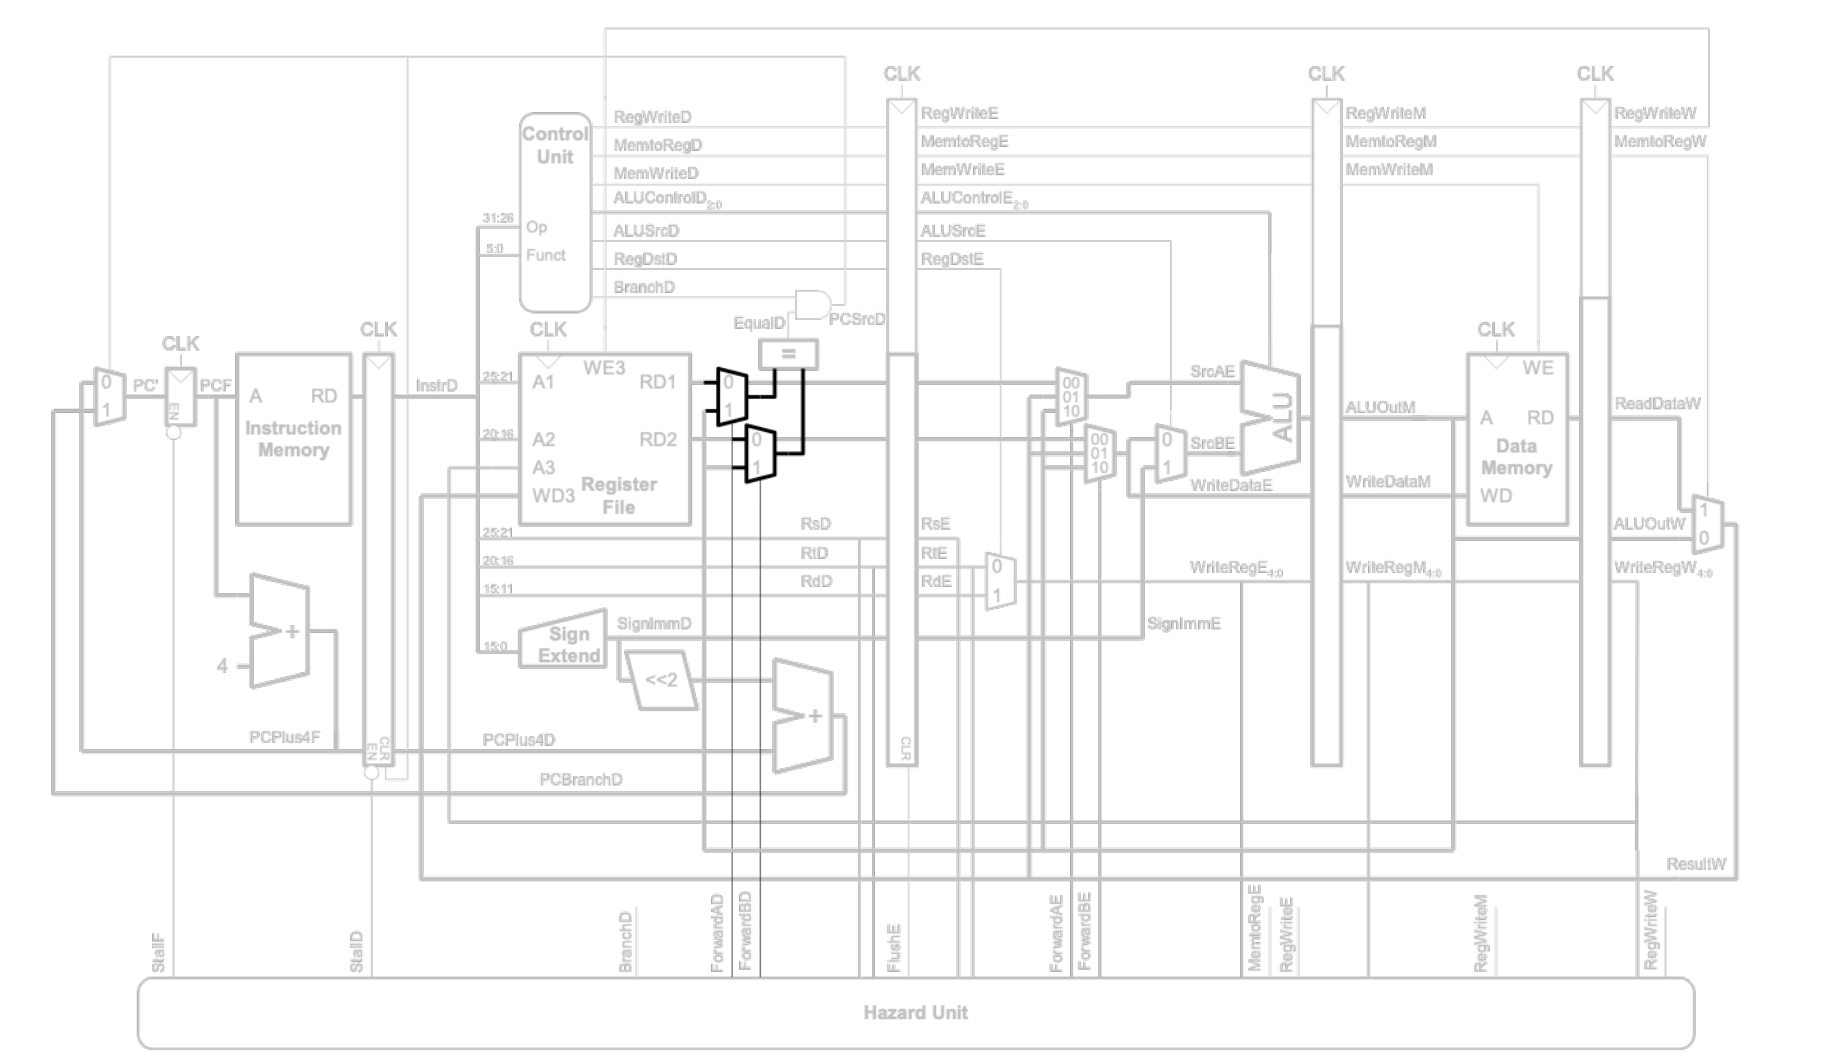
\includegraphics[width=0.75\textwidth]{figure/解决控制冒险的数据通路.png}
	\caption{解决控制冒险的数据通路}
	\label{fig:control_hazard_data_path}
\end{figure}
控制冒险的逻辑控制如下:
\begin{lstlisting}[language=Verilog,caption={控制冒险逻辑控制},label={lst:control_hazard_logic}]
	assign forwardAD = ((rsD != 0) && (rsD == writeregM) && regwriteM);
	assign forwardBD = ((rtD != 0) && (rtD == writeregM) && regwriteM);
	
	// --------------------------------
	// stall
	wire lwstall;
	//stallF, stallD, flushE;
	wire branchstall;
	assign lwstall = ((rsD == rtE) || (rtD == rtE)) && memtoregE; // . 判断 decode 阶段 rs 或 rt 的地址是否是 lw 指令要写入的地址;
	assign branchstall = branchD && regwriteE && 
						   (writeregE == rsD || writeregE == rtD) ||
						   branchD && memtoregM &&
						   (writeregM == rsD || writeregM == rtD);
	
	assign stallF = lwstall || branchstall;
	assign stallD = lwstall || branchstall;
	assign flushE = lwstall || branchstall;
\end{lstlisting}
\subsubsection{接口定义}
% \textcolor{red}{接口定义请使用表格,需要包括\textbf{接口信号名、方向、宽度、含义}(红字为内容说明,请删除)}

% \begin{table}[htp]
% \caption{接口定义模版}\label{tab:signaldef}
% \begin{center}
% 	\begin{tabular}{|l|l|l|p{6cm}|}
% 	\hline
% 	\textbf{信号名} & \textbf{方向} & \textbf{位宽} & \textbf{功能描述}\\ \hline \hline
% 	valid			& Output& 1-bit & If CPU stopped or any exception happens, valid signal is set to 0.\\ 
% 	\hline
% 	\end{tabular}
% \end{center}
% \end{table}

\begin{table}[H]
	\caption{接口定义}\label{tab:signaldef}
	\begin{center}
	\begin{tabular}{lllp{6cm}}
	\hline
	\textbf{信号名} & \textbf{方向} & \textbf{位宽} & \textbf{功能描述} \\ \hline \hline
	rst & Input & 1-bit & 重置信号 \\ \hline
	rsD & Input & 5-bit & decoder 阶段的 rs 号码 \\ \hline
	rtD & Input & 5-bit & decoder 阶段的 rt 号码 \\ \hline
	rsE & Input & 5-bit & execute 阶段的 rs 号码 \\ \hline
	rtE & Input & 5-bit & execute 阶段的 rt 号码 \\ \hline
	regwriteE & Input & 1-bit & execute 阶段的寄存器写使能 \\ \hline
	regwriteM & Input & 1-bit & memory access 阶段的寄存器写使能 \\ \hline
	regwriteW & Input & 1-bit & writeback 阶段的寄存器写使能 \\ \hline
	memtoregE & Input & 1-bit & execute 阶段指令是否需要将数据读写至寄存器 \\ \hline
	memtoregM & Input & 1-bit & memory 阶段指令是否需要将数据读写至寄存器 \\ \hline
	branchD & Input & 1-bit & decoder 阶段判断是否为分支指令 \\ \hline
	writeregE & Input & 5-bit & execute 阶段的寄存器写号码 \\ \hline
	writeregM & Input & 5-bit & memory 阶段的寄存器写号码 \\ \hline
	writeregW & Input & 5-bit & writeback 阶段的寄存器写号码 \\ \hline
	forwardAE & Output & 2-bit & execute 阶段由 mux3 选择 SrcA \\ \hline
	forwardBE & Output & 2-bit & execute 阶段由 mux3 选择 SrcB \\ \hline
	forwardAD & Output & 2-bit & decoder 阶段由 mux3 选择 SrcA \\ \hline
	forwardBD & Output & 2-bit & decoder 阶段由 mux3 选择 SrcB \\ \hline
	stallF & Output & 1-bit & fetch 阶段停滞 \\ \hline
	stallD & Output & 1-bit & decoder 阶段停滞 \\ \hline
	flushE & Output & 1-bit & 清空 execute 阶段状态 \\ \hline
	\end{tabular}
	\end{center}
	\end{table}

% \section{实验过程记录}

\subsection{问题 1: 触发器的使能端问题}
问题描述:实验中 Controller 模块用到的流水线寄存器不含有使能端,datapath 模块使用的流
水线寄存器含有使能端,刚开始实验时混淆。

解决方案:Controller 模块使用的流水线寄存器为 floprc,即含有 rst 和 clear 信号的触发器,因
为此处流水线寄存器的功能只是在时钟信号到来时将数据传入或接受输入的控制信号,随时有
效,无需使能端;datapath 使用的流水线寄存器存储的是数据信号,只有在使能端有效的情况下才
输入输出。
\subsection{问题 2: 触发器的使能端问题}
问题描述:连接 datapath 时,判断需要分支时直接将当前 PC 值与 branch 字节地址相加。但
实际上此时的 PC 已经执行了 PC+4,存在偏移。

解决方案:在计算 branch 分支地址时将 PC-4 再传入。
\subsection{问题 3: 触发器的使能端问题}
问题描述:流水线寄存器的 rst 和 clear 看似作用相同,都是清空流水线实则不同

解决方案:。rst 相当于整个电路的开关,置 1 时整个电路归零,有可能是异常或流水线冲突;
clear 是较为简单的流水线清空,有可能是人为清空流水线结束 CPU 或者流水线地址跳转却已经
执行跳转前代码。因此需将 rst 和 clear 分开。

% \section{实验结果及分析}
% \textcolor{red}{需要仿真图一张,控制台打印输出图一张,要求仿真图中包含pc、instr、rs、rt、rd、result信号,仿真图应在控制台打印输出Simulation succeeded时截图。控制台打印输出图为此时截图。}
\subsection{仿真图}
\begin{figure}[H]
    \centering
    \caption{仿真图}
    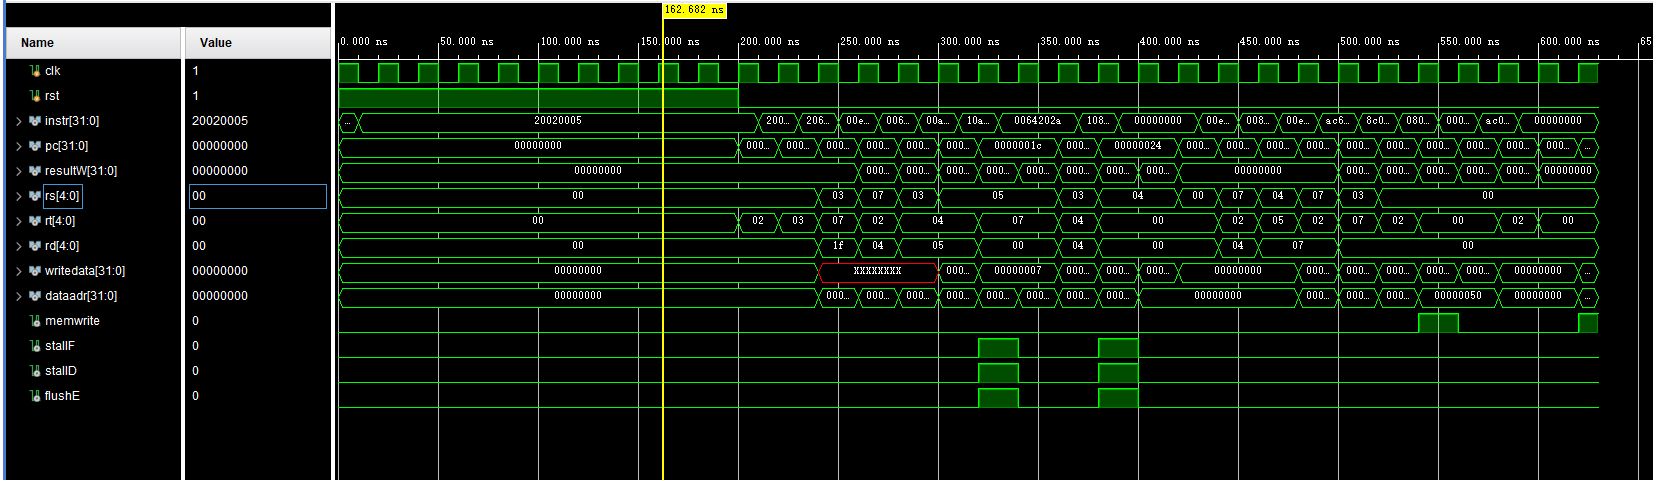
\includegraphics[width=1\textwidth]{figure/仿真.png}
    \label{fig:sim}
\end{figure}
\subsection{控制台}
\begin{figure}[H]
    \centering
    \caption{控制台输出}
    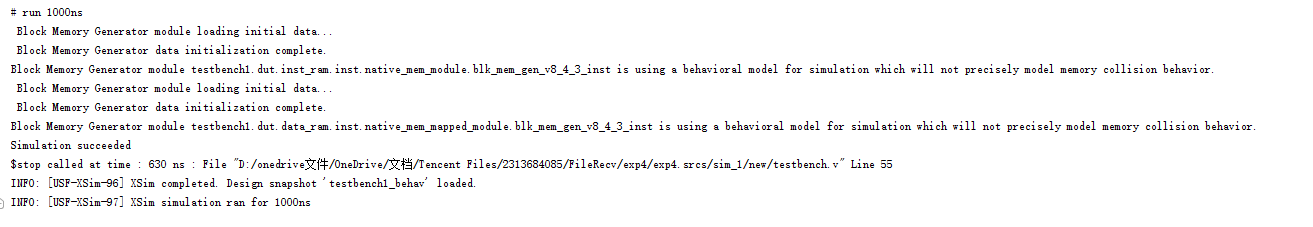
\includegraphics[width=1\textwidth]{figure/控制台.png}
    \label{fig:console}
\end{figure}
\subsection{仿真结束}
\begin{figure}[H]
    \centering
    \caption{仿真结束}
    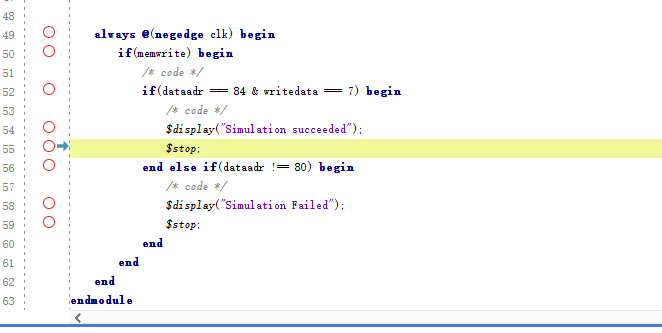
\includegraphics[width=0.8\textwidth]{figure/仿真结束.png}
    \label{fig:sim_stop}
\end{figure}

\appendix
\section{test}

\begin{table}[h]
    \centering
    \begin{tabular}{ccccc}
        \hline
        \textbf{Debris} & \textbf{Longitude} & \textbf{Latitude} & \textbf{Altitude (m)} & \textbf{Time (s)} \\ \hline
        1 & 110.457995 & 27.681618 & 798.4 & 95.30 \\ 
        2 & 110.488570 & 27.656313 & 777.6 & 95.53 \\ 
        3 & 110.479030 & 27.679734 & 1685.8 & 97.38 \\ 
        4 & 110.490165 & 27.609234 & 8768.6 & 99.21 \\ \hline
    \end{tabular}
    \caption{Debris Data}
    \label{tab:debris}
\end{table}

\end{document}
